\section{Visualization demo}

\subsection{Show motion track}

If you are new to the concepts of rotation and translation, you may find that their form looks complicated, because after all, each expression can be converted to other ways, and the conversion formula is sometimes longer. However, although the values of the rotation matrix and transformation matrix may not be intuitive enough, we can easily draw them in the window.

In this section we demonstrate two visual examples. First, let's say that we recorded the trajectory of a robot in some way, and now I want to draw it into a window. Suppose the track file is stored in trajectory.txt, and each line is stored in the following format: $$ \mathrm {time}, t_x, t_y, t_z, q_x, q_y, q_z, q_w, $$ where $ \mathrm {time} $ refers The recording time of this pose, $ \bm {t} $ is translation, $ \bm {q} $ is the rotation quaternion, all recorded in the world coordinate system to the robot coordinate system. Below we read these tracks from the file and display them in a window. In principle, if you just talk about "robot pose", then you can use $ \bm {T}_{WR} $ or $ \bm {T}_{RW} $ , in fact they are only one inverse. It means that knowing one of them makes it easy to get another. If you want to store \textbf {robot's track}, then you can store $ \bm {T}_{WR} $ at all timesOr $ \bm {T}_{RW} $ , which doesn't make much difference.

When drawing the trajectory, we can draw the "trajectory" into a sequence of points, which is similar to the "trajectory" we imagined. Strictly speaking, this is actually the \textbf {the coordinates of the origin of the robot (camera) coordinate system in the world coordinate system}. Consider the origin of the robot coordinate system, ie $ \bm {O}_{R} $ , then the $ \bm {O}_{W} $ at this time is the coordinates of the origin in the world coordinate system:
\begin{equation}
\ bm {O} _ {W} = \ bm {T} _ {WR} \ bm {O} _R = \ bm {t} _ {WR}.
\end{equation}
This is the translation part of $ \bm {T}_{WR} $ . So, you can see \textbf {where the camera is} directly from $ \bm {T}_{WR} $ , which is why we say $ \bm {T}_{WR} $ is more intuitive. Therefore, in the visualization program, the track file stores $ \bm {T}_{WR} $ instead of $ \bm {T}_{RW} $ .

Finally, we need a library that supports 3D drawing. There are many libraries that support 3D drawing, such as the familiar matlab, python matplotlib, OpenGL and so on. In linux, a common library is OpenGL-based Pangolin library \footnote { \url {https://github.com/stevenlovegrove/Pangolin}}, which provides some GUI based on the support of OpenGL drawing operations. Features. In the second edition of the book, we used git's submodule feature to manage the third-party libraries that this book relies on. Readers can go directly to the 3rdparty folder to install the required libraries, and git guarantees that I am consistent with the version you are using.

\begin{lstlisting}[language=c++,caption=slambook2/ch3/examples/plotTrajectory.cpp]
#include <pangolin/pangolin.h>
#include <Eigen/Core>
#include <unistd.h>

using namespace std;
using namespace Eigen;

// path to trajectory file
string trajectory_file = "./examples/trajectory.txt";

void DrawTrajectory(vector<Isometry3d, Eigen::aligned_allocator<Isometry3d>>);

int main(int argc, char **argv) {
    vector<Isometry3d, Eigen::aligned_allocator<Isometry3d>> poses;
    ifstream fin(trajectory_file);
    if (!fin) {
        cout << "cannot find trajectory file at " << trajectory_file << endl;
        return 1;
    }
    
    while (!fin.eof()) {
        double time, tx, ty, tz, qx, qy, qz, qw;
        fin >> time >> tx >> ty >> tz >> qx >> qy >> qz >> qw;
        Isometry3d Twr(Quaterniond(qw, qx, qy, qz));
        Twr.pretranslate(Vector3d(tx, ty, tz));
        poses.push_back(Twr);
    }
    cout << "read total " << poses.size() << " pose entries" << endl;
    
    // draw trajectory in pangolin
    DrawTrajectory(poses);
    return 0;
}

void DrawTrajectory(vector<Isometry3d, Eigen::aligned_allocator<Isometry3d>> poses) {
    // create pangolin window and plot the trajectory
    pangolin::CreateWindowAndBind("Trajectory Viewer", 1024, 768);
    glEnable(GL_DEPTH_TEST);
    glEnable(GL_BLEND);
    glBlendFunc(GL_SRC_ALPHA, GL_ONE_MINUS_SRC_ALPHA);
    
    pangolin::OpenGlRenderState s_cam(
    pangolin::ProjectionMatrix(1024, 768, 500, 500, 512, 389, 0.1, 1000),
    pangolin::ModelViewLookAt(0, -0.1, -1.8, 0, 0, 0, 0.0, -1.0, 0.0)
    );
    
    pangolin::View &d_cam = pangolin::CreateDisplay()
        .SetBounds(0.0, 1.0, 0.0, 1.0, -1024.0f / 768.0f)
        .SetHandler(new pangolin::Handler3D(s_cam));
    
    while (pangolin::ShouldQuit() == false) {
        glClear(GL_COLOR_BUFFER_BIT | GL_DEPTH_BUFFER_BIT);
        d_cam.Activate(s_cam);
        glClearColor(1.0f, 1.0f, 1.0f, 1.0f);
        glLineWidth(2);
        for (size_t i = 0; i < poses.size(); i++) {
            // draw three axes of each pose
            Vector3d Ow = poses[i].translation();
            Vector3d Xw = poses[i] * (0.1 * Vector3d(1, 0, 0));
            Vector3d Yw = poses[i] * (0.1 * Vector3d(0, 1, 0));
            Vector3d Zw = poses[i] * (0.1 * Vector3d(0, 0, 1));
            glBegin(GL_LINES);
            glColor3f(1.0, 0.0, 0.0);
            glVertex3d (Ow [0], Ow [1], Ow [2]);
            glVertex3d (Xw [0], Xw [1], Xw [2]);
            glColor3f(0.0, 1.0, 0.0);
            glVertex3d (Ow [0], Ow [1], Ow [2]);
            glVertex3d (Is [0], Is [1], Is [2]);
            glColor3f(0.0, 0.0, 1.0);
            glVertex3d (Ow [0], Ow [1], Ow [2]);
            glVertex3d (Zw [0], Zw [1], Zw [2]);
            glEnd();
        }
        // draw a connection
        for (size_t i = 0; i < poses.size(); i++) {
            glColor3f(0.0, 0.0, 0.0);
            glBegin(GL_LINES);
            auto p1 = poses[i], p2 = poses[i + 1];
            glVertex3d(p1.translation()[0], p1.translation()[1], p1.translation()[2]);
            glVertex3d(p2.translation()[0], p2.translation()[1], p2.translation()[2]);
            glEnd();
        }
        pangolin::FinishFrame();
        usleep(5000);   // sleep 5 ms
    }
}
\end{lstlisting}

This program demonstrates how to draw a 3D pose in Panglin. We draw the three axes of each pose in red, green, and blue (actually we calculate the world coordinates of each axis), and then connect the traces with black lines. The program runs as shown in \autoref {fig:trajectory}.

\begin{figure}[!htp]
    \centering
    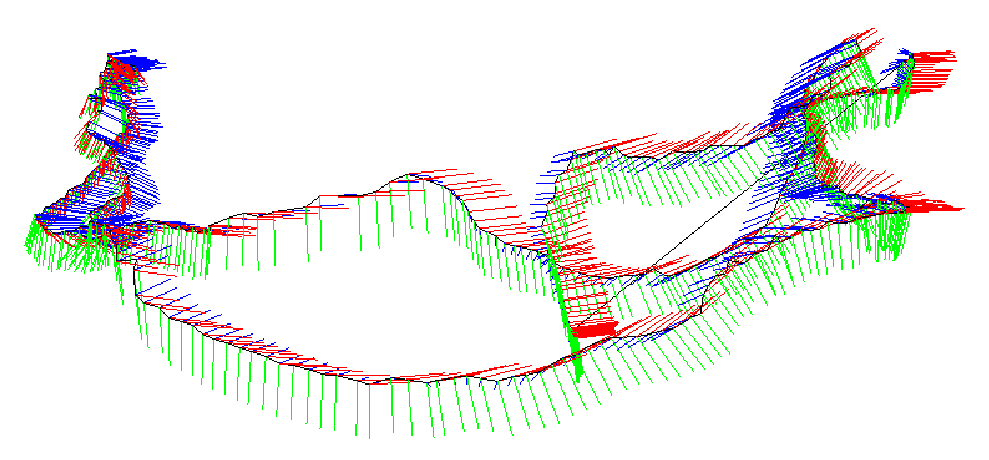
\includegraphics[width=0.8\textwidth]{chapter03/rigidMotion/trajectory.pdf}
    \caption {Results of pose visualization}
    \label{fig:trajectory}
\end{figure}

\subsection {Show camera pose}
\begin{figure}[!htp]
    \centering
    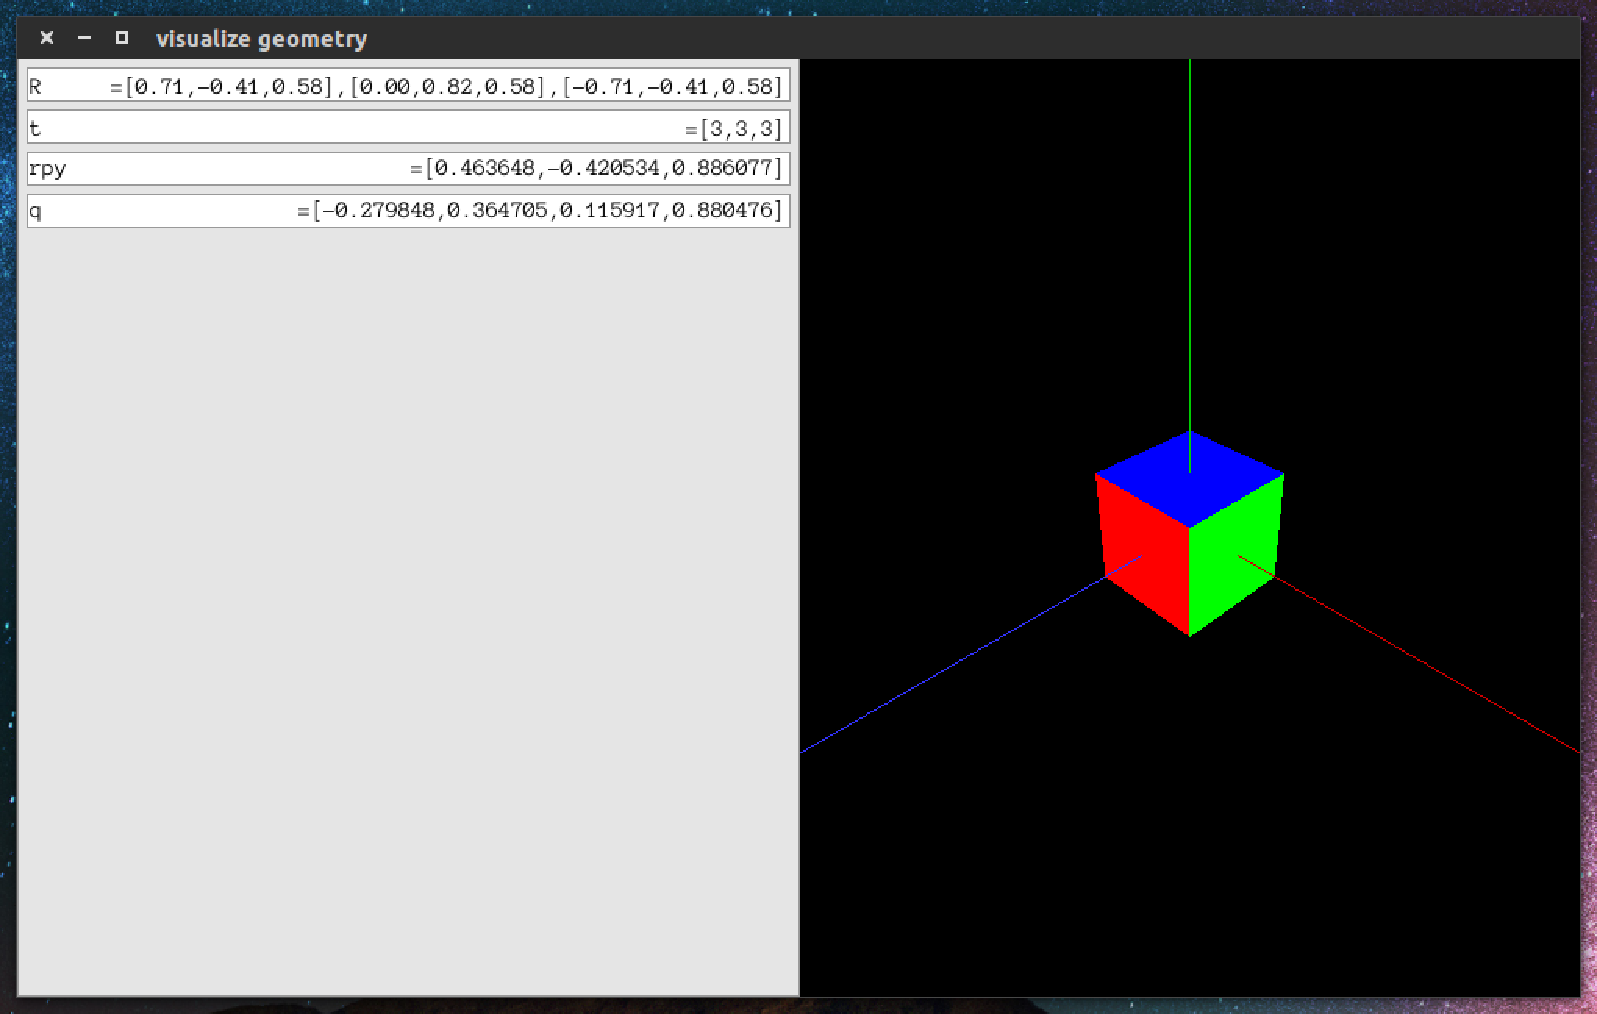
\includegraphics[width=0.8\textwidth]{chapter03/rigidMotion/visualizeGeometry.pdf}
    \ caption { Visualization program for rotation matrix, Euler angle, quaternion. }
    \label{fig:visualizeGeometry}
\end{figure}

In addition to displaying the trajectory, we can also display the pose of the camera in the 3D window. In slambook2/ch3/visualizeGeometry, we visualize various expressions of camera poses (see \autoref{fig:visualizeGeometry}). When the reader uses the mouse to operate the camera, the box on the left side will display the rotation matrix, translation, Euler angle and quaternion of the camera pose in real time. You can see how the data changes. According to our experience, you should not see their intuitive meaning except for the Euler angle. However, although the rotation matrix or transformation matrix is not intuitive, it is not difficult to visually display them. This program uses the Pangolin library as a 3D display library. Please refer to Readme.txt to compile the program.
